\chapter{Benchmark Architecture and Design}
\label{cha:middle}

%This chapter presents the fundamental process of development and execution of The Benchmark, from the energy model used to the tests performed. Thus, Section \ref{sc:enerymodel} defines an energy model that we consider essential to achieve a ea model. Then, in Chapter \ref{sc:dbtest} it will be presented the DBMS under test and their reasons to be included in this study.  In Chapter \ref{sc:Design} it is given the tests made and an explanation for their designs. Finally, in Chapter \ref{sc:execution} it is present the execution of this study.


This Chapter presents the necessary steps of our methodology to measure and compare different \gls{dbms}. Section \ref{sc:enerymodel} defines the energy model that supports our methods. Afterward, in Section \ref{sc:dbtest}, we present the \gls{dbms} we consider in our study.  Then, Section \ref{sc:Design} describes the design of the benchmarks we defined. Finally, in Section \ref{sc:execution}, we show their execution process.


\section{Energy Measure Method}

\label{sc:enerymodel}

Before deciding the energy model we consider in our benchmark of the \gls{dbms}, it is essential to understand that the overall energy consumption of software systems divides into two groups: consumption when idle and dynamic consumption (that is, consumption when running). 

As mention in Section~\ref{energypower}, , idle consumption represents the energy needed for the system to run on minimal usage without any interference of user activity. Dynamic consumption is the energy consumed by a task or activity triggered by the user, where this energy is the difference between total consumption and idle consumption. Thus, the total energy consumed by the following equation:

\begin{equation}
E_{Total} = E_{Idle} + E_{Dynamic}
\end{equation}$
$

Where $E_{Total}$ represents the total energy consumed by the software system consumption,  $E_{Idle}$ the idle consumption, and $E_{Dynamic}$ the dynamic consumption.

\paragraph{Idle Consumption:} Idle consumption is the base consumption needed to ensure that the system is ready. It is obtained by measuring the energy consumption of the system during an interval of time. During which the system remains running with the lowest possible activity and without any user interference. 

Using the frameworks mentioned in Section~\ref{energyframe}. It is possible to divide the $E_{Idle}$ subgroups that we define as relevant in Section~\ref{relevant}. The following equation presents these subgroups:

\begin{equation}
E_{Idle} = E_{Idle\_Others} + ( E_{Idle\_CPU} + E_{Idle\_DRAM} + E_{Idle\_DISK})
\end{equation}$
$

Where $E_{Idle\_CPU}$ represents the energy consumed by the \gls{cpu} when the software is in an idle model, $E_{Idle\_DRAM}$ the idle consumption of the main memory, $E_{Idle\_DISK}$ the idle consumption of the disk, and $E_{Idle\_Others}$ represent the remaining energy consumed.

As mention in Section~\ref{sc:RAPL} , the $E_{Idle\_CPU}$ and $E_{Idle\_DRAM}$ can be estimated by \gls{rapl}. For measuring the $E_{Idle\_DISK}$, we will use the Arduino method mentioned in Section~\ref{arduino}.

By using the \gls{rapl} Package estimation metric, which includes \gls{cpu}, and \gls{gpu}, the following equation can be an alternative definition for the total consumption in idle mode:


\begin{equation}
\label{eq:iddlepackage}
E_{Idle} = E_{Idle\_Others} + ( E_{Idle\_Package} + E_{Idle\_DRAM} + E_{Idle\_DISK})
\end{equation}$
$

\paragraph{Dynamic Consumption:} The dynamic energy consumption can only be determined after we have measured the idle consumption. Only then can we distinguish between idle and the energy impacts caused by the user. In this phase, any slight increase in the overall energy counts towards the dynamic consumption. Very much like in idle mode, this consumption must divide into the same groups. The following equation represents this separation :

\begin{equation}
E_{Dynamic} = E_{Dynamic\_CPU} + E_{Dynamic\_DRAM} + E_{Dynamic\_DISK}
\end{equation}$
$

As for the idle consumption, the  $E_{Dynamic\_CPU}$ and $E_{Dynamic\_DRAM}$  can be measure with \gls{rapl}, and the  $E_{Dynamic\_DISK}$ by the Arduino. To obtain these values, we need to remove the idle consumption of the total consumption in those components. Thus, for each subsystem, the equations are as follows:


\begin{equation}
E_{Dynamic\_CPU} =  E_{Total\_CPU} - E_{idle\_CPU}
\end{equation}$
$

\begin{equation}
E_{Dynamic\_DRAM} =  E_{Total\_DRAM} - E_{idle\_DRAM}
\end{equation}$
$

\begin{equation}
E_{Dynamic\_DISK} =  E_{Total\_DISK} - E_{idle\_DISK}
\end{equation}$
$


As in Equation~\ref{eq:iddlepackage}, \gls{cpu} and \gls{gpu} can be estimated together by the Package metric. The dynamic consumption also translates into the following equation:

\begin{equation}
E_{Dynamic\_Package} =  E_{Total\_Package} - E_{idle\_Package}
\end{equation}$
$

\begin{equation}
\label{eq:DDYNAMICpackage}
E_{Dynamic} = E_{Dynamic\_Others} + ( E_{Dynamic\_Package} + E_{Dynamic\_DISK} + E_{Dynamic\_DRAM})
\end{equation}$
$

Through these analyzes, it is to conclude that idle consumption is not relevant to compare different \gls{dbms} on the same system since it is a static value. Therefore, we decided only to show and compare the dynamic energy consumption of all measurements in Chapter \ref{cha:Results}  for a better and easier understanding of the results obtained. 


\section{Databases Under Test}
\label{sc:dbtest}


In our digital information age, where more and more information (only) exists in digital form (see, for example: how photography evolved in the last two decades), databases are a vital part of all types and organization sizes (from small to large)~\cite{10.14778/2732240.2732246}. Moreover, data centers are also becoming an increasingly critical part of the infrastructure in our digitalized society. As a consequence of the concern with energy expenditure, a company/software engineer needs to understand their scenario and select the fitting DBMS that combines runtime performance with energy efficiency.

Although there is extensive (research) work on analyzing and benchmarking the runtime performance of DBMS\cite{10.14778/1920841.1920902,seybold2019mowgli,stonebraker2010mapreduce,10.1145/2452376.2452448}, there is still a lack of knowledge on the energy efficiency of the different DBMS that supports the data centers. In this thesis, we decide to compare four well-known and widely used DBMS: \textit{MySQL}, \textit{MariaDB}, \textit{Postgres}, and \textit{Redis}. Our decision on the DBMS was also based on whether the HammerDB supported it.

\subsection{MySQL}

The first DBMS chosen was MySQL. MySQL is the most popular open-source relational DBMS in the market and is known for providing high-performance, robust SQL, multi-threaded, multi-user access to several databases. Allan Larsson and Michael Widenius created MySQL in 1995, and now it is owned by Oracle Corporation. Some of its customers include GitHub, Uber, NASA, Tesla, Netflix. 

MySQL's other features are: high compatibility, high portability, usage of fast B-tree disk tables with index compression, provides transactional and nontransactional storage engines, thread-based memory allocation system, optimized nested-loop join, in-memory hash tables used for temporary tables, and other things.

\subsection{MariaDB}

Another DBMS chosen was MariaDB. MariaDB is a popular open-source relational DBMS. The original developers of MySQL in 2009 made MariaDB ensure a free and open-source DBMS. Originally designed as an enhanced, drop-in replacement for MySQL, MariaDB is a fast, scalable, and many other tools that make it very versatile for a wide variety of use cases.

Since MariaDB is built on top of the latest version of MySQL, it has most of the features of MySQL and high compatibility between them. MariaDB provides some improvements from MySQL like more Storage Engines, some Speed Improvements like parallel replication, better testing, and other things.

\subsection{Postgres}

The last relational DBMS chosen was Postgres. Postgres is an open-source object-relational DBMS that uses and extends the SQL language combined with many features that safely store and scale the most complicated data workload. PostgreSQL started its development in 1986 at the University of California and has more than 30 years of active development on the core platform.

PostgreSQL's main attraction is its architecture, consistency, data integrity, robust feature set, extensibility, and the open-source community's commitment to delivering efficiency and creative solutions consistently. PostgreSQL is currently used in several research applications and comes with several add-ons, such as the popular PostGIS geospatial database extender. PostGIS is widely used for geographic data, and in many universities, they use as an educational tool due to its open-source code. It has some object-oriented features, such as inheritance and custom types, in addition to the characteristics of a relational DBMS.


\subsection{Redis}

The last DBMS chosen was Redis. Redis is an open-source non-relational DBMS of the type key-value that supports in-memory data structure store, used as a database, cache, and message broker \cite{da2015redis}.
Redis is a well-established open-source project, and many companies use Redis like Twitter, Tumblr, Instagram, Flick, and The New York Times. Redis is one of the most popular non-relational DBMS in the market\cite{da2015redis}.
Redis is known for its fast key-value database that stores a mapping of keys to five types of values: strings, lists, sets, hashes, sorted sets \cite{10.55552505464,redis}. It supports in-memory persistent storage at the disk, replication to scale read performance, and client-side sharding to scale write performance. Depending on the use case, the persisted data are either periodically dumped to disk or appending each command to a disk-based log. Redis also provides asynchronous replication\cite{10.55552505464,redis}. 

Additionally, Redis has configurable key expiration, transaction, and publish/subscribe features. It also provides Lua scripting to create new commands. With these tools, it makes a very versatile database\cite{da2015redis,redis}.

\section{Design}
\label{sc:Design}
%HammerDB

%We decide to use HammerDB as it is a benchmark tool that can replicate the behavior of most cloud-based applications as a service, verify comprehensive performance and multiple metrics in a simple real-world environment on a virtual environment with virtual users~\cite{hammerdb}.

%Another reason we choose HammerDB was for the automated software testing~\cite{hammerdb} so we can configure how many times the HammerDB will run and how many virtual users that he will use and for how long it will run, providing at the end of every execution the \gls{tpm} and the \gls{nopm}. With these numbers and the energy spent, we can have ample information to answer the RQ2, and with an adjustable number of users, it can assist in the RQ3.

We decided to use HammerDB as a benchmark tool that can replicate the behavior of the most cloud-based applications as a service, verify comprehensive performance and multiple metrics in a simple real-world environment on a virtual environment with \gls{vu}~\cite{hammerdb}. Another reason was the automated software testing \cite{hammerdb} so we can configure how many times the HammerDB will run and how many \gls{vu} it will use, and for how long it will run, providing at the end of every execution the \gls{tpm} and the \gls{nopm}. With these numbers and the energy spent, we can have ample information to answer the \textbf{RQ2}, and with an adjustable number of users, it can assist in the \textbf{RQ3}.


%Cenarios

%The initial step to obtaining comparable results about the energy consumed in each DBMS is to define a configuration for HammerDB for each scenario . 
 
 The initial step to obtaining comparable results about the energy consumed in each \gls{dbms} is to define a configuration for HammerDB for each scenario. 
 
 
 %-> Explicar Numero  X   de utilizadores: 1, 8, 32, 12X,

%With the Research Question mentioned in Section \ref{sc:rq}, many scenarios can be deducted. These scenarios are differentiated by the number of users that we want to run in the system. So, we decide to go with four different scenarios of server participation. The first case is a server running with the lowest users possible, so we execute the benchmark with only one virtual use. A second scenario is a small group of users practicing on the server, so we run with eight virtual users. The third scenario is a simulation of the server on intensive work with a big group of users, and for that, we use 64 virtual users. The final scenario is the server saturated with users, and for that, we decide with 128 virtual users. 
%While the first scenario is enough to answer the \textbf{RQ1} and \textbf{RQ2}, the \textbf{RQ3} needs the other three scenarios.


With the Research Question mentioned in Section \ref{sc:rq}, we can deduce various scenarios. The number of users we run in the system differentiates these scenarios. So, we decide to go with four different scenarios of server participation. The first case is a server running with the lowest users possible, so we execute the benchmark with only 1 \gls{vu}. A second scenario is a small group of users practicing on the server, so we run with 8 \gls{vu}. The third scenario is a simulation of the server doing intensive work with a big group of users, and for that, we use 64 \gls{vu}. The final one is the server saturated with users, and for that, we decide with 128 \gls{vu}. 
While the first scenario is enough to answer \textbf{RQ1} and \textbf{RQ2}, the \textbf{RQ3} needs the others.
%configuration
 

 
 For each of them, we created a script for each \gls{dbms}.  These scripts must simulate the behavior of daily usage of a \gls{dbms}. So using a custom script inside the HammerDB was out of the question, and we decided to use the \gls{tpcc} benchmark. We decide to do one warehouse in every scenario to simplify this study, with the intention in future work to expand to more warehouses. 
 
%EXPLICAR AS WAREHOUSES

To simplify this study, we decide to do one warehouse in every scenario with the intention of future work to expand this study to more warehouses. 

%EXPLICAR O RAM UP

%Then we must decide on the time that the benchmark builds up the transaction rate by caching data in the buffer cache database before the benchmark is executed. This known as the rampup time. In our study e decide to set ramup to 1/5 of the execution time~\cite{hammerdb}.


Then we must decide on the time that the benchmark builds up the transaction rate by caching data in the buffer cache database before the benchmark is executed. This is known as the rampup time. In our study, we decide to set the ramup to 1/5 of the execution time~\cite{hammerdb}.

%tempo 
For greater precision and adequate replication of various usage scenarios, each case was performed with 5, 10, and 30 minutes.



%Final note
Finally, in addition to the previous scripts, we also created a script that would remove idle consumption from the measured energy consumption using a previous measured idle consumption.



% Falar aqui apesar de terem sido feitos, nao foram aprofundados porque os resultos são bastante parecidos


%In Chapter \ref{cha:Results}, it is presented and discuss only the 5m tests. Even with most of the 10 and 30 minutes results measured, they aren't discussed here due to their conclusions being very similar to the conclusions of 5 minutes. These results are able in the annex.

It is presented and discussed in Chapter \ref{cha:Results} only the 5 minutes tests. Even with most of the 10 and 30 minutes results measured, they weren't discussed here due to their conclusions being very similar to the conclusions of 5 minutes. These results are available in the annex of this document.





\section{Execution}
\label{sc:execution}




%DESENHO DA ARQUITETURA DO Sistema.

Figure \ref{fig:arch} shows the execution of the benchmark and measurements of energy consumption of \gls{dbms}, where it displays the architecture of our energy benchmarking system and the flow of actions.



%Imagem
\begin{figure}[H]
  \centering
  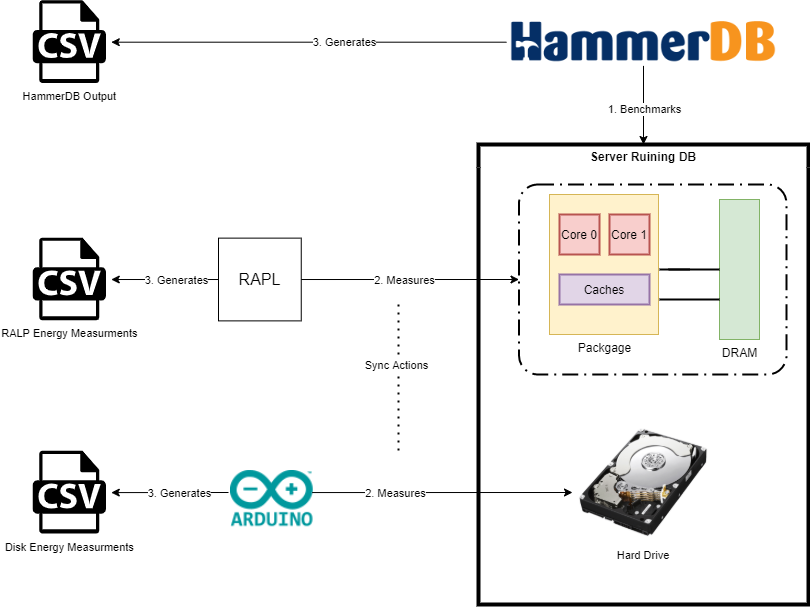
\includegraphics[width=\linewidth]{Chapters/images/arquitetura.png}
      \caption{Benchmark Architecture and flow of events}
  \label{fig:arch}
\end{figure}

% Explicar 1º Passo% cada script foi executado 10 vezes



As seen in Figure \ref{fig:arch}, the first action of our execution is the Benchmark initialization and execution of HammerDB. To obtain proper and reliable energy readings, we needed to diminish the effects of cold starts, warm-ups, cache effects, and other effects that may influence energy consumption. So, each scenario is executed ten times with a sleep time of 2 minutes between each execution.

%In order to have proper energy readings, we need to reduce the effects of cold starts, warm-ups, cache effects, and other effects that may influence energy consumption. Thus, each script is executed 10 times with a sleep time of 2 minutes between each execution.


%Sample do Arduino e RAPL

Immediately after the start of the Benchmark execution, The measurements of the energy consumption start. The framework tools used were the ones mentioned in Section \ref{energyframe}.  In the case of the \gls{rapl}, the sample used was 100 measurements per second, and for the Arduino was ten measures per second.

%Explicar o RAPLSERVER que foi usado para sync as mediçoes entre o Arduino e o RAPL.

These two measurement tools are in sync throughout the entire execution. We accomplished this by using a C program that starts two independent sync threads: one that accesses the \gls{rapl} to measure the \gls{cpu} is power consumption, and the other accesses the Arduino to measure the disk's power consumption. They are active during the execution of HammerDB and accumulate energy readings in static arrays to limit their computing overhead.


%3fase

The third and final phase of our execution begins after the HammerDB execution is completed. This step saves each measurement mad in its respective CSV file for further analysis.



%Para reduzir os vestigios e faciltar montar diferentes dbms foi usado DOCKER


Also, for each database, we decide to use dockers containers because it is a solution that simplifies the setup by providing a pre-built image that is portable, simple to maintain, and providing a facility to automate the applications when they are deployed into containers~\cite{rad2017introduction,10.1145/2723872.2723882}. Although several studies recognize that dockers provide an overhead in running these containers~\cite{chung2016using,varghese2016container,impactDocker,felter2015updated}, dockerized benchmarks can be acceptable when comparing different database systems if the idle consumption values are disregarded~\cite{grambow2019safe}.


%System Configuration
\paragraph{System Configuration}

We ran this study on a server with the following specifications presented in Table  \ref{Tab:physicalserver}, this consists of an Intel(R) Core i5-4460 3.28 GHz \gls{cpu}, 16 GB of \gls{ram}, 250 GB \gls{hdd}, and operating system Ubuntu 16.10 . A detailed overview of the \gls{cpu} is in Table \ref{tab:cpuspec} and for Second Storage is in Table \ref{tab:diskspec}.

\begin{table}[H]
\centering
\begin{tabular}{|c|c|}
\hline
Hardware               & Model \\ \hline
CPU                    & Intel(R) Core i5-4460 3.28 GHz   \\ \hline
Operation System       & Ubuntu 16.10   \\ \hline
Ram Size               & 16G   \\ \hline
Secondary Storage      & Hitachi Travelstar 250 GB   \\ \hline
\end{tabular}
\caption{Physical server specifications}
\label{Tab:physicalserver}

\end{table}

    \begin{table}[!ht]
    \centering
\begin{minipage}[t]{0.48\linewidth}\centering
\begin{tabular}{|c|c|}
\hline
\multicolumn{2}{|c|}{CPU}      \\ \hline
Brand               & Intel    \\ \hline
Model               & i5-4460  \\ \hline
Microarchitecture   & Haswell  \\ \hline
Number of cores     & 4        \\ \hline
Clock Speed         & 3.20 GHz \\ \hline
Max Turbo Frequency & 3.40 GHz \\ \hline
Cache               & 6 MB     \\ \hline
Interface           & Sata 3   \\ \hline
Buffer Size         & 8MB      \\ \hline
\end{tabular}
\caption{Specifications of CPU used}\label{tab:cpuspec}
\end{minipage}\hfill%
\begin{minipage}[t]{0.48\linewidth}\centering
\begin{tabular}{|c|c|}
\hline
\multicolumn{2}{|c|}{Second Storage} \\ \hline
Brand          & Hitachi GST         \\ \hline
Model          & HTE543225A7A384     \\ \hline
Series         & Travelstar Z5K320   \\ \hline
Type           & HDD                 \\ \hline
Capacity       & 250 GB              \\ \hline
RPM            & 5400                \\ \hline
Interface      & Sata 3              \\ \hline
Buffer Size    & 8MB                 \\ \hline
\end{tabular}
\caption{Specifications of Disk used}\label{tab:diskspec}
\end{minipage}
\end{table}

%

\begin{table}[H]
\centering
\begin{tabular}{|c|c|}
\hline
\multicolumn{2}{|c|}{CPU}      \\ \hline
Brand               & Intel    \\ \hline
Model               & i5-4460  \\ \hline
Microarchitecture   & Haswell  \\ \hline
Number of cores     & 4        \\ \hline
Clock Speed         & 3.20 GHz \\ \hline
Max Turbo Frequency & 3.40 GHz \\ \hline
Cache               & 6 MB     \\ \hline
Interface           & Sata 3   \\ \hline
Buffer Size         & 8MB      \\ \hline
\end{tabular}
\caption{Specifications of CPU used}\label{tab:cpuspec}

\end{table}


%
\begin{table}[H]
%https://www.newegg.com/hitachi-gst-travelstar-z5k320-250gb-hte543225a7a384/p/N82E16822145458
\centering
\begin{tabular}{|c|c|}
\hline
\multicolumn{2}{|c|}{Second Storage} \\ \hline
Brand          & Hitachi GST         \\ \hline
Model          & HTE543225A7A384     \\ \hline
Series         & Travelstar Z5K320   \\ \hline
Type           & HDD                 \\ \hline
Capacity       & 250 GB              \\ \hline
RPM            & 5400                \\ \hline
Interface      & Sata 3              \\ \hline
Buffer Size    & 8MB                 \\ \hline
\end{tabular}
\caption{Specifications of Disk used}\label{tab:diskspec}

\end{table}

This system has no additional software installed or running other than required to run this research. Additionally, we had the caution to use the most recent and compatible version of all external software used here at the time of the measurements. So listed in Table \ref{Tab:softwareconfig} are all the versions used.

\begin{table}[H]
\centering
\begin{tabular}{|c|c|}
\hline
Software & Version \\ \hline
Redis    &  5.0.5  \\ \hline
Postgres &  11.5   \\ \hline
MySQL    &  8.0    \\ \hline
MariaDB  &  10.0      \\ \hline
HammerDB  &  3.2   \\ \hline
Docker & 19.03.11 \\ \hline
\end{tabular}
\caption{Software Configuration on physical server}
\label{Tab:softwareconfig}

\end{table}





All software artifacts shown in Figure~\ref{fig:arch} and mention in this chapter, are  available as a public repository at \url{https://github.com/greensoftwarelab/GreenSGDBS}.
